\section{Filtro passabanda e post amplificatore}
	Per la realizzazione del filtro passabanda e del post amplificatore
	sono stati realizzati rispettivamente  il circuito in \figurename{ \ref{fig:banda}} ,impiegando le relative componentistiche, ed il circuito in \figurename{ \ref{fig:post}}.
	\begin{figure}[h]
		\begin{minipage}{0.75\textwidth}
		\begin{minipage}{0.75\textwidth}
			\centering
			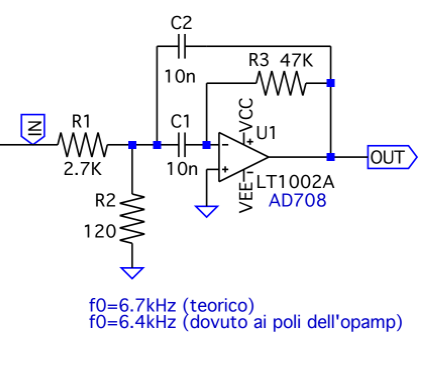
\includegraphics[width=\textwidth]{banda.png}
			\caption{Filtro passabanda e post amplificatore}
			\label{fig:banda}
		\end{minipage}
		\begin{minipage}{0.19\textwidth}
			\begin{tabular}{l@{ }c@{ }l}
				$R_{1}$& = &\SI{2.66(3)}{\kilo\ohm}\\
				$R_{2}$& = &\SI{0.118(1)}{\kilo\ohm}\\
				$R_3$& = &\SI{46.4(5)}{\kilo\ohm}\\
			\end{tabular}
		\end{minipage}
		\end{minipage}
		\begin{minipage}{0.75\textwidth}
		\begin{minipage}{0.75\textwidth}
			\centering
			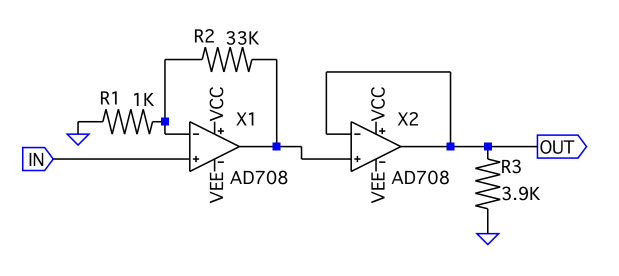
\includegraphics[width=\textwidth]{post.png}
			\caption{Filtro passabanda e post amplificatore}
			\label{fig:post}
		\end{minipage}
		\begin{minipage}{0.19\textwidth}
			\begin{tabular}{l@{ }c@{ }l}
				$R_{1}$& = &\SI{0.972(9)}{\kilo\ohm}\\
				$R_{2}$& = &\SI{33.1(4)}{\kilo\ohm}\\
				$R_3$& = &\SI{3.87(4)}{\kilo\ohm}\\
			\end{tabular}
		\end{minipage}
	\end{minipage}
	\end{figure}
	\paragraph{Verifica passa-banda }
	Per la misura della risposta in frequenza del filtro passa-banda
	è stata campionato il guadagno del circuito in risposta a dei segnali 
	sinusoidali di varia frequenza. Si riportano i dati campionati in \tablename{ \ref{tab:1}}.
	\begin{table}[h]
		\begin{tabular}{sss}
			
		\end{tabular}
	\end{table}
	
	